\chapter{Introduzione} 
% \note{levare capitolo 1 come titolo}
\linespread{1.5}

\section{In Breve}
In questa sezione vengono introdotti: lo scopo e lo svolgimento del tirocinio compreso il contesto in cui è stato svolto il lavoro, l'applicazione Livesignage e la sua architettura, lo stato dell'arte e gli obiettivi raggiunti. Infine è presentata una descrizione della struttura di questa relazione.

\section{Scopo del tirocinio}

Il tirocinio è stato svolto presso l'azienda Softhrod srl. di Volterra all'interno dell'applicazione Livesignage per la distribuzione di contenuti multimediali targettizzati. Lo scopo del tirocinio è l'analisi, la progettazione e lo sviluppo di un'applicazione lato client per il sistema operativo WebOS Signage sui dispositivi LG:  display professionali, videowall, smart TV, sistemi IoT, media player. L'applicazione deve essere in grado di mostare specifici contenuti multimediali sulla base di eventi acquisiti dall'ambiente circostante, come ad esempio condizioni metereologiche o orario, e parametri indicati dall'utente. L'applicazione è stata sviluppata in linguaggio JavaScript sfruttando le API REST messe a disposizione dal sistema operativo.

\section{Modalità di lavoro}

Ho lavorato in modalità mista ( telematica e presenza ) in maniera prevalentemente autonoma, ma mantenendo un confronto diretto sia con gli altri sviluppatori sia con i progettisti per tutte le scelte riguardanti le logiche e lo sviluppo dell'applicazione. Ho così avuto modo di capire quale sia il processo produttivo dell'azienda, come si lavora in team e l'attenzione per l'esperienza utente, fondamentale per questo ambito.

\section{Digital signage e Livesignage}

Il digital signage è una forma di comunicazione direttamente nel punto vendita, in spazi pubblici aperti o all'interno di edifici, anche nota in Italia come segnaletica digitale, videoposter o cartellonistica digitale, i cui contenuti vengono mostrati ai destinatari attraverso schermi elettronici o videoproiettori disposti in maniera strategica. Le tipologie di contenuti che possono essere mostrati sono molteplici: video, mappe, immagini, menù, feed real time, elementi interattivi; di conseguenza sono molteplici i contesti in cui può essere utilizzato: negozi, ristoranti, alberghi e totem nelle città sono alcuni esempi.

Livesignage è un’applicazione per il digital signage sviluppata per vari dispositivi specializzati tra i quali quelli di Samsung. L’idea è quella di fornire all'utente un modo semplice e flessibile per creare i propri contenuti cercando, quando possibile, di automatizzare il processo usando tutte le informazioni contenute sul suo sito web o sul proprio database. Tramite l'utilizzo di alcuni plug-in, è possibile ampliare ancora le feature disponibili: come la possibilità di fare webcall e l'integrazione delle informazioni reperibili dai propri social network.

Inoltre, alla creazione di una playlist (vedi sezione \ref*{statoarte}), viene automaticamente creata una progressive Web App: un'applicazione navigabile direttamente dal browser e completamente impostabile dal creatore dei contenuti permettendo un'interazione maggiore dell'utente finale.

La Figura \ref{fig:liveToursitSample} illustra un esempio di quello che potrebbe essere mostrato su un totem installato in una città; tramite il codice QR creato automaticamente insieme ai contenuti mostrati, il consumatore può quindi ricevere le informazioni in modo più dettagliato sul proprio dispositivo mobile senza bisogno di scaricare applicazioni o fare ricerche online.

\begin{figure}[!htb]
    \centering
    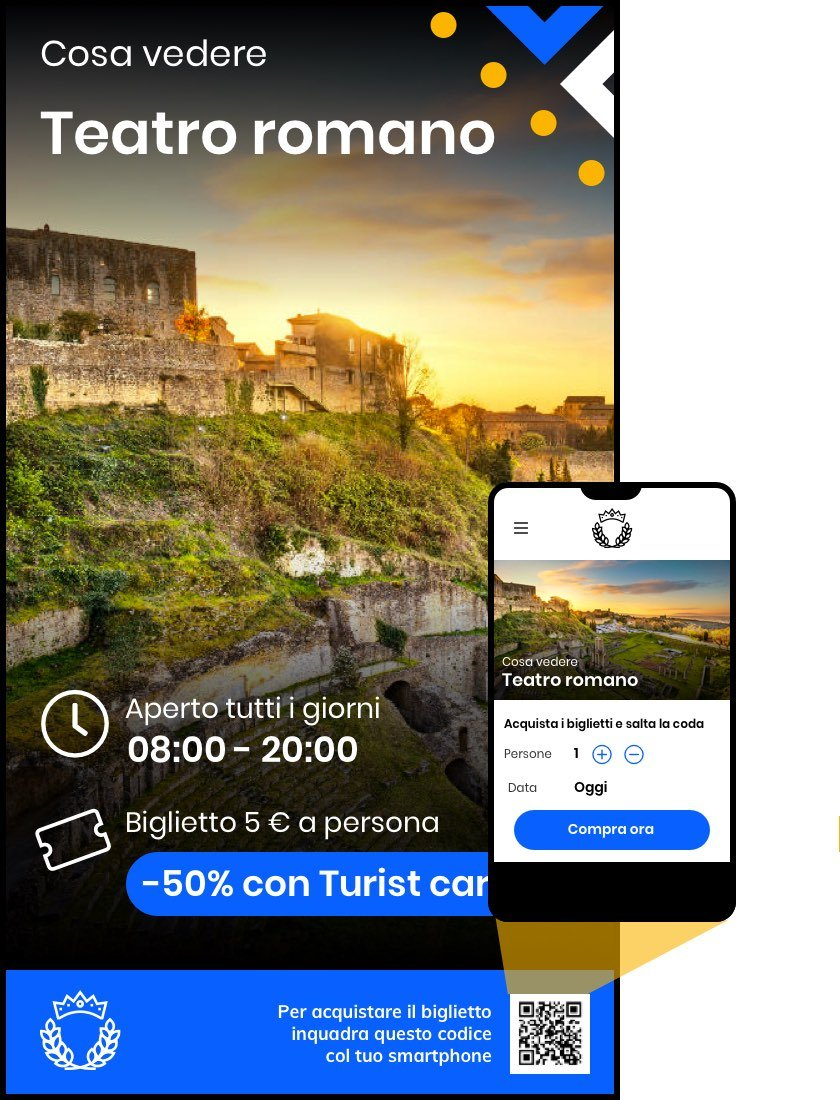
\includegraphics[width= 0.5\textwidth]{images/Introduzione/LiveTurist.jpg} 
    \caption{Esempio di infografica in un'installazione cittadina.} 
    \label{fig:liveToursitSample}
\end{figure}



\section{Stato dell'arte}\label{statoarte}

All'inizio del tirocinio il client di Livesignage era già disponibile per dispositivi di Samsung e Raspberry.  

L'idea alla base dell'applicazione è quella di mostrare una serie di slide organizzate in playlist; ogni slide può mostrare diversi tipi di contenuti come ad esempio immagini, video, web page, mappe, notizie, input esterni (ad esempio telecamere e fogli di calcolo). Le playlist possono essere di diverso tipo:

\begin{itemize}
    \item Semplici: le slide vengono mostrate a schermo intero e si susseguono continuamente;
    \item Composte: in questo caso lo spazio a disposizione viene suddiviso in più parti e in ognuna di queste viene mostrata una playlist diversa (Fig. \ref*{fig:playlist-composta});
    \item Concatenate: vengono concatenate più playlist una dopo l'altra.
    \begin{figure}[!htb]
        \centering
        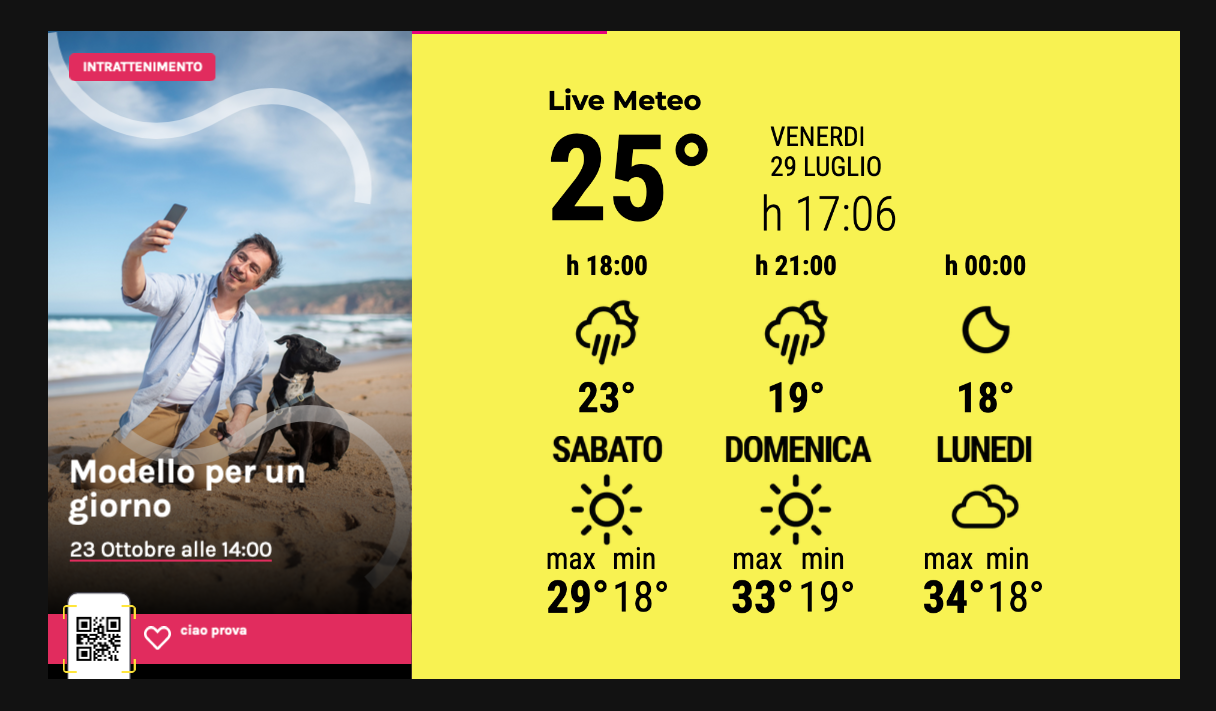
\includegraphics[width= 0.8\textwidth]{images/Introduzione/playlist-composta.png} 
        \caption{Una playlist composta.} 
        \label{fig:playlist-composta}
    \end{figure}
\end{itemize}


Oltre alle playlist è possibile utilizzare dei plug-in per poter dare al cliente più possibilità di personalizzazione. Ad esempio permettendo di  mostrare contenuti interattivi utilizzando l'input dell'utente tramite il touchscreen o di inserire il proprio e-commerce.

\subsection{Architettura}
\begin{figure}[H]
    \centering
    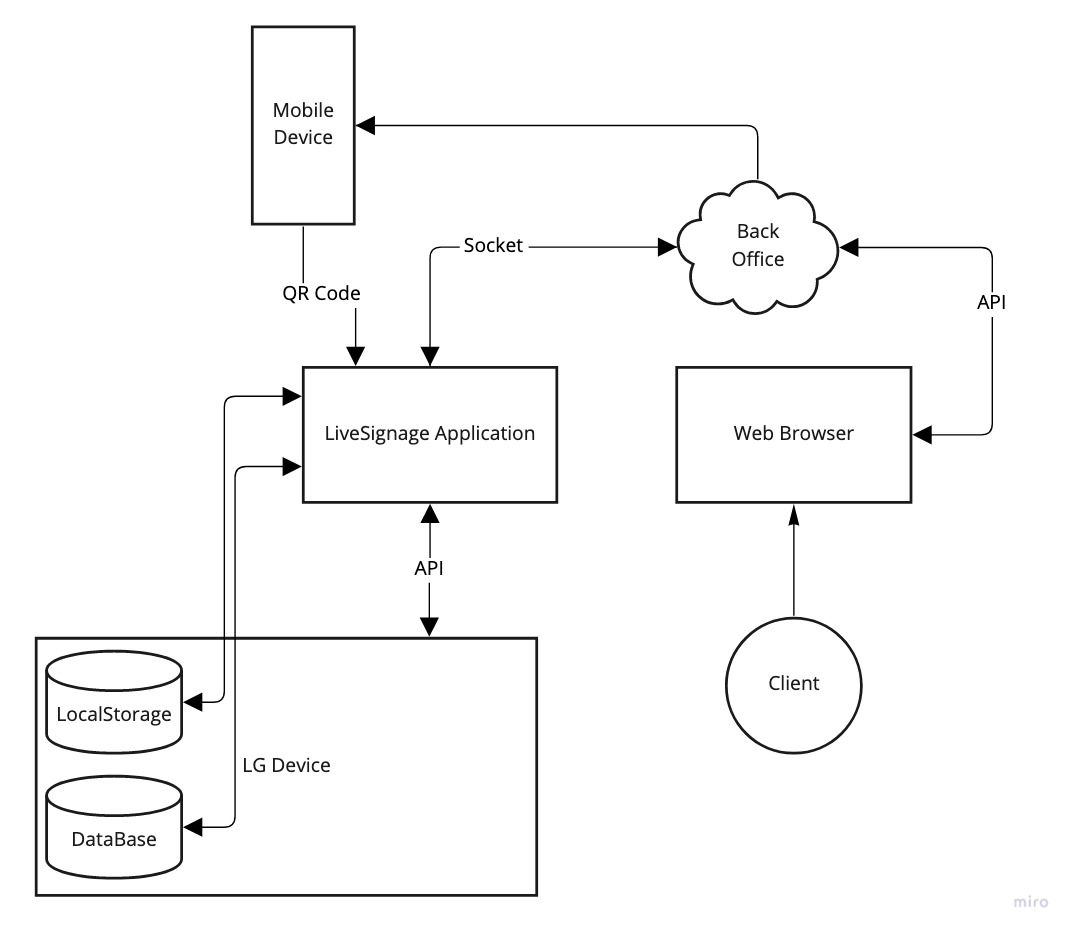
\includegraphics[width= 1.1\textwidth]{images/Introduzione/Architettura.jpg} 
    \caption{Architettura dell'applicazione.} 
    \label{fig:architettura}
\end{figure}

L'applicazione è suddivisa in due parti: una parte è installata sul dispositivo per il digital signage, questa si occupa di riceve dal back office le playlist da mostrare e le impostazioni che il creatore di contenuti ha impostato (timer di accensione, volume, luminosità), la seconda parte, il back office, è online ed è accessibile tramite una web page (Fig: \ref*{fig:schermata-web}): qui è possibile controllare alcune funzioni del device client, creare e impostare le proprie playlist e i plug-in. 

\begin{figure}[H]
    \centering
    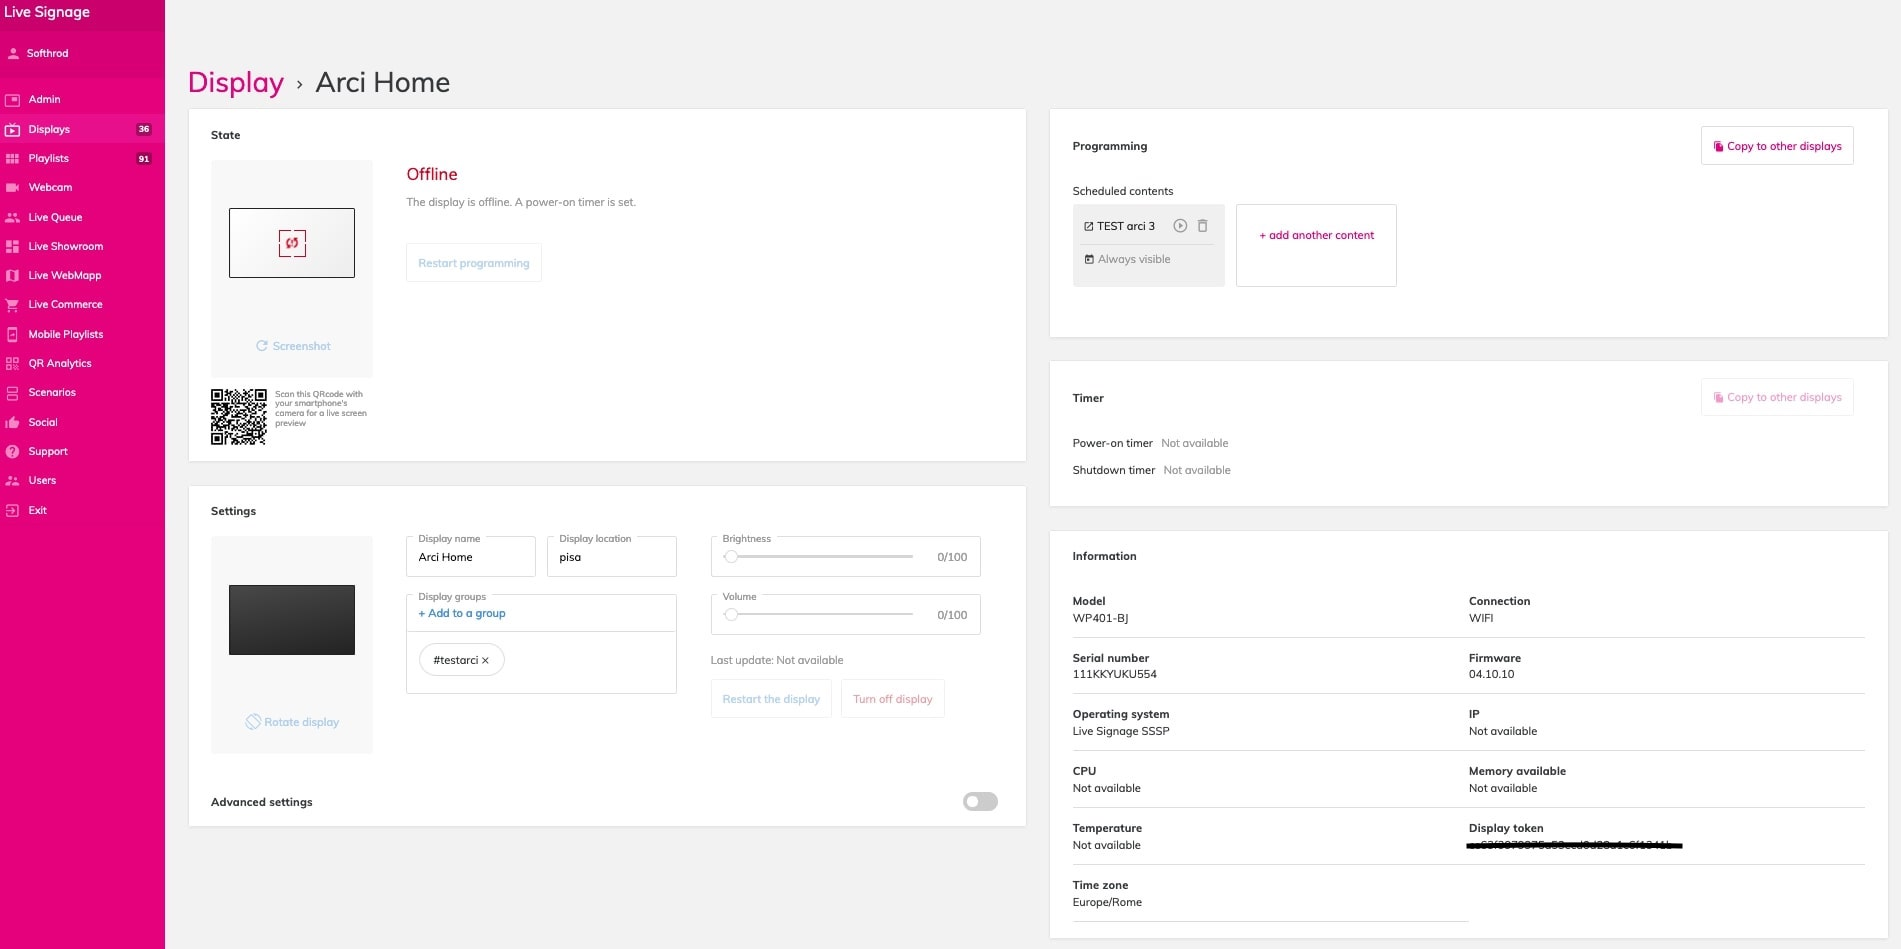
\includegraphics[width= 1.1\textwidth]{images/Introduzione/SchermataWebLS.jpg} 
    \caption{Schermata del portale online per programmare il display.} 
    \label{fig:schermata-web}
\end{figure}

Le modifiche impostate dal back office vengono comunicate al dispositivo che, tramite le interfacce offerte dal sistema, scrive i file necessari alla persistenza delle informazioni come ad esempio le playlist create , scarica i contenuti multimediali necessari e configura le impostazioni selezionate del creatore di contenuti.

La figura \ref*{fig:architettura} mostra in maniera schematica l'architettura dell'applicazione e l'interazione con il consumatore.

Nella figura \ref*{fig:use_case} sono rappresentati i passaggi necessari alla creazione di una playlist, l'invio di questa al dispositivo selezionato dal creatore di contenuti e l'interazione con l'utente finale.

\begin{figure}[H]
    \centering
    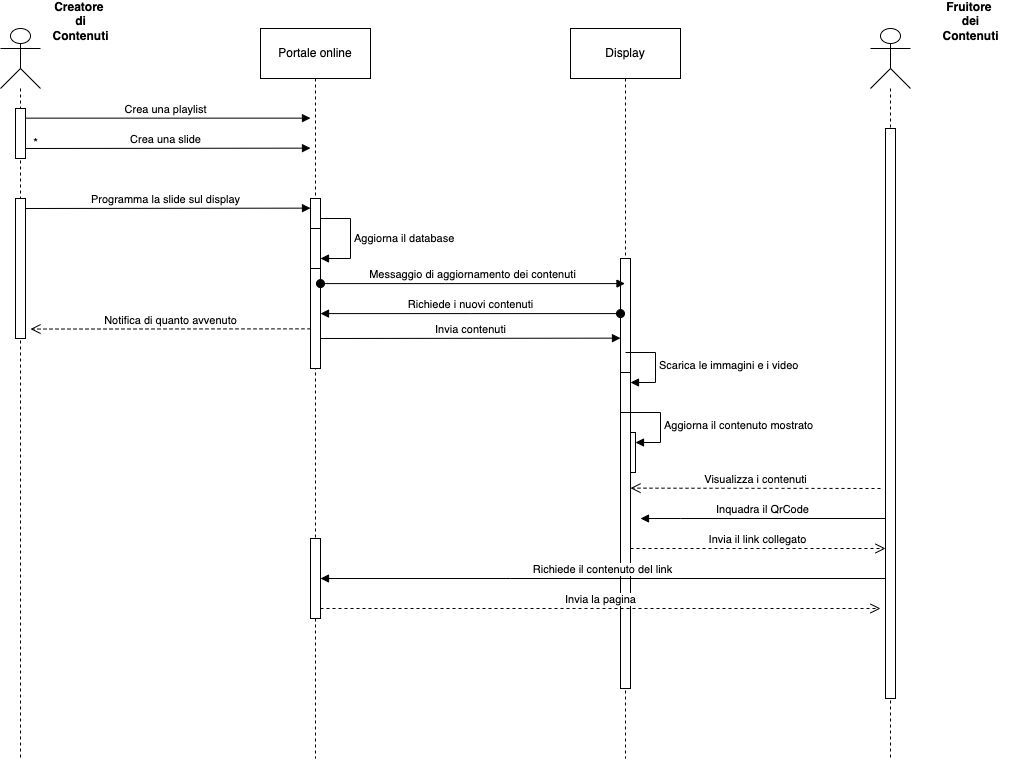
\includegraphics[width= 1.1\textwidth]{images/Introduzione/diagramma_flusso.png} 
    \caption{Creazione di una playlist.} 
    \label{fig:use_case}
\end{figure}


% \note{figura web page piú grande}

\section{Requisiti}
Lo svolgimento del lavoro è incentrato sullo sviluppo di un'applicazione client per dispositvi di digital signage, sviluppata su sistema operativo WebOS Signage di LG; questa deve essere in grado di mostrare contenuti multimediali tramite l'uso di HTML e CSS su un web engine, installato sul device, basato su Chromium, deve poter eseguire degli script JavaScript, aprire una socket di comunicazione verso il web server, scaricare le immagini e i video necessari alla corretta visualizzazione dei contenuti programmati e comunicare con il sistema operativo del device tramite l'uso delle interfacce messe a disposizione dal sistema operativo.
L'applicazione deve inoltre poter salvare in memoria i contenuti e le informazioni necessarie affinchè possa funzionare anche in assenza di connessione. Deve infine poter modificare il comportamento di alcuni tasti del telecomando durante l'esecuzione.


\section{Obiettivi raggiunti}

Al termine del tirocinio la versione di Livesignage per WebOS Signage è stata correttamente sviluppata; ho avuto inoltre modo di aggiungere, o almeno studiare la possibilità di farlo, alcune funzionalità non presenti nella versione per dispositivi Samsung. Queste non erano previste a inizio tirocinio ma sono state pensate a seguito dello studio della documentazione.

\section{Struttura della relazione}
Di seguito una breve descrizione della suddivisione in capitoli di questa relazione.
\begin{itemize}
    \item Tecnologie utilizzate: Descrizione delle tecnologie a disposizione, loro differenze e scelte implementative da queste derivanti. Linguaggi e librerie utilizzate.
    \item Livesignage su WebOS: Descrizione del lavoro svolto, difficoltà incontrate e soluzioni trovate, modifiche all'applicazione pre-esistente. Descrizione della fase di testing finale.
    \item Studio di funzionalità aggiuntive: In questo capitolo si presenta una descrizione della fase di analisi e, quando possibile, aggiunta delle nuove funzionalità e alcune idee per possibili miglioramenti futuri.
    \item Conclusioni: Riassunto dei punti principali affrontati e degli obiettivi raggiunti. Competenze acquisite.
\end{itemize}